\documentclass{ctexart}
\usepackage{tikz}
\usepackage{float}
\usetikzlibrary{shapes.geometric, arrows, positioning}
\title{小车预习}
\author{何铭源}
\date{\today}
\begin{document}
\maketitle
\section{目标检测}
通过小车摄像头,计算目标小球的重心位置,和能够框住小球的矩形长宽。并计算小车与小球的距离是否合适。
\section{路径规划}
通过计算小球所被包含的矩形长宽,计算小车与小球的距离,并通过小球距离画面中心的距离,来判断小车的行驶方向并进行行驶。

此时需要考虑抓取小球的时候小球并不在画面中心,而机械臂是在小球的正前方。
\section{机械臂抓取}
云台角度校准:通过向导程序调整云台水平/垂直舵机确保摄像头正对目标。
机械臂动作:
\begin{enumerate}
    \item 机械臂调整至预设舵机角度。
    \item 机械爪张开并贴近目标物体。
    \item 闭合机械爪抓取物体后抬升。
\end{enumerate}
\section{其他动作抓拍}
\begin{figure}[H]
    \centering
    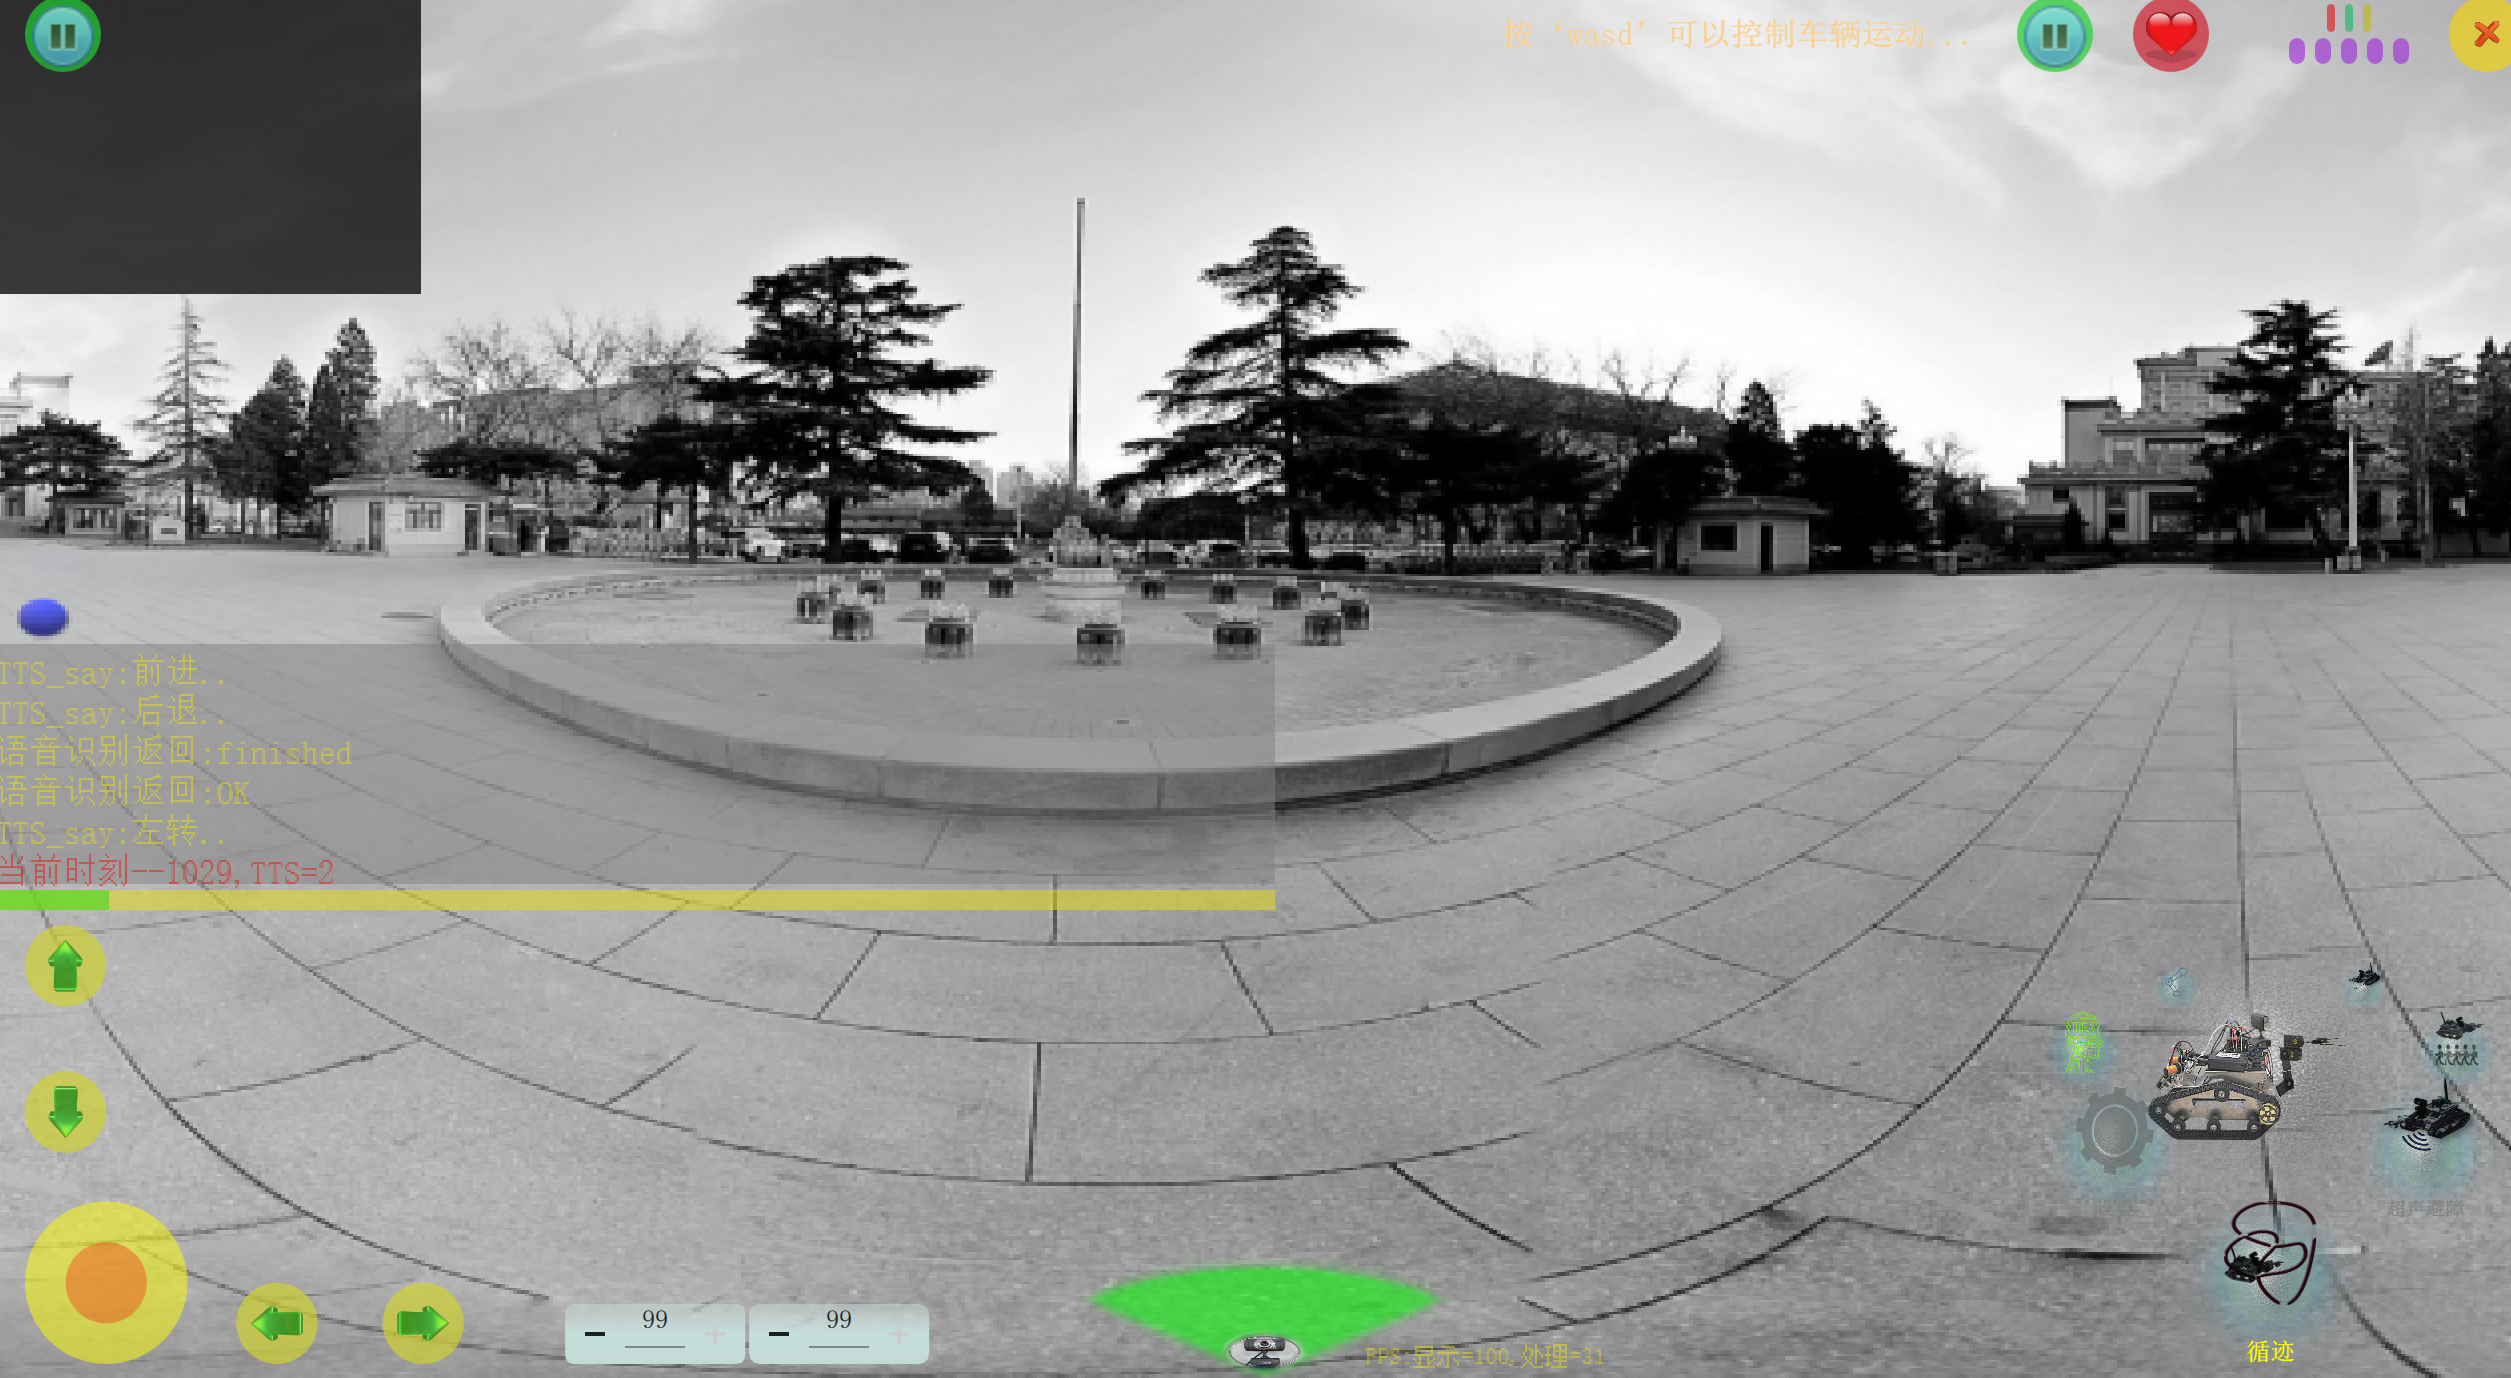
\includegraphics[width = .8\textwidth]{./figure/前后左右.png}
    \caption{基本动作}
\end{figure}
\begin{figure}[H]
    \centering
    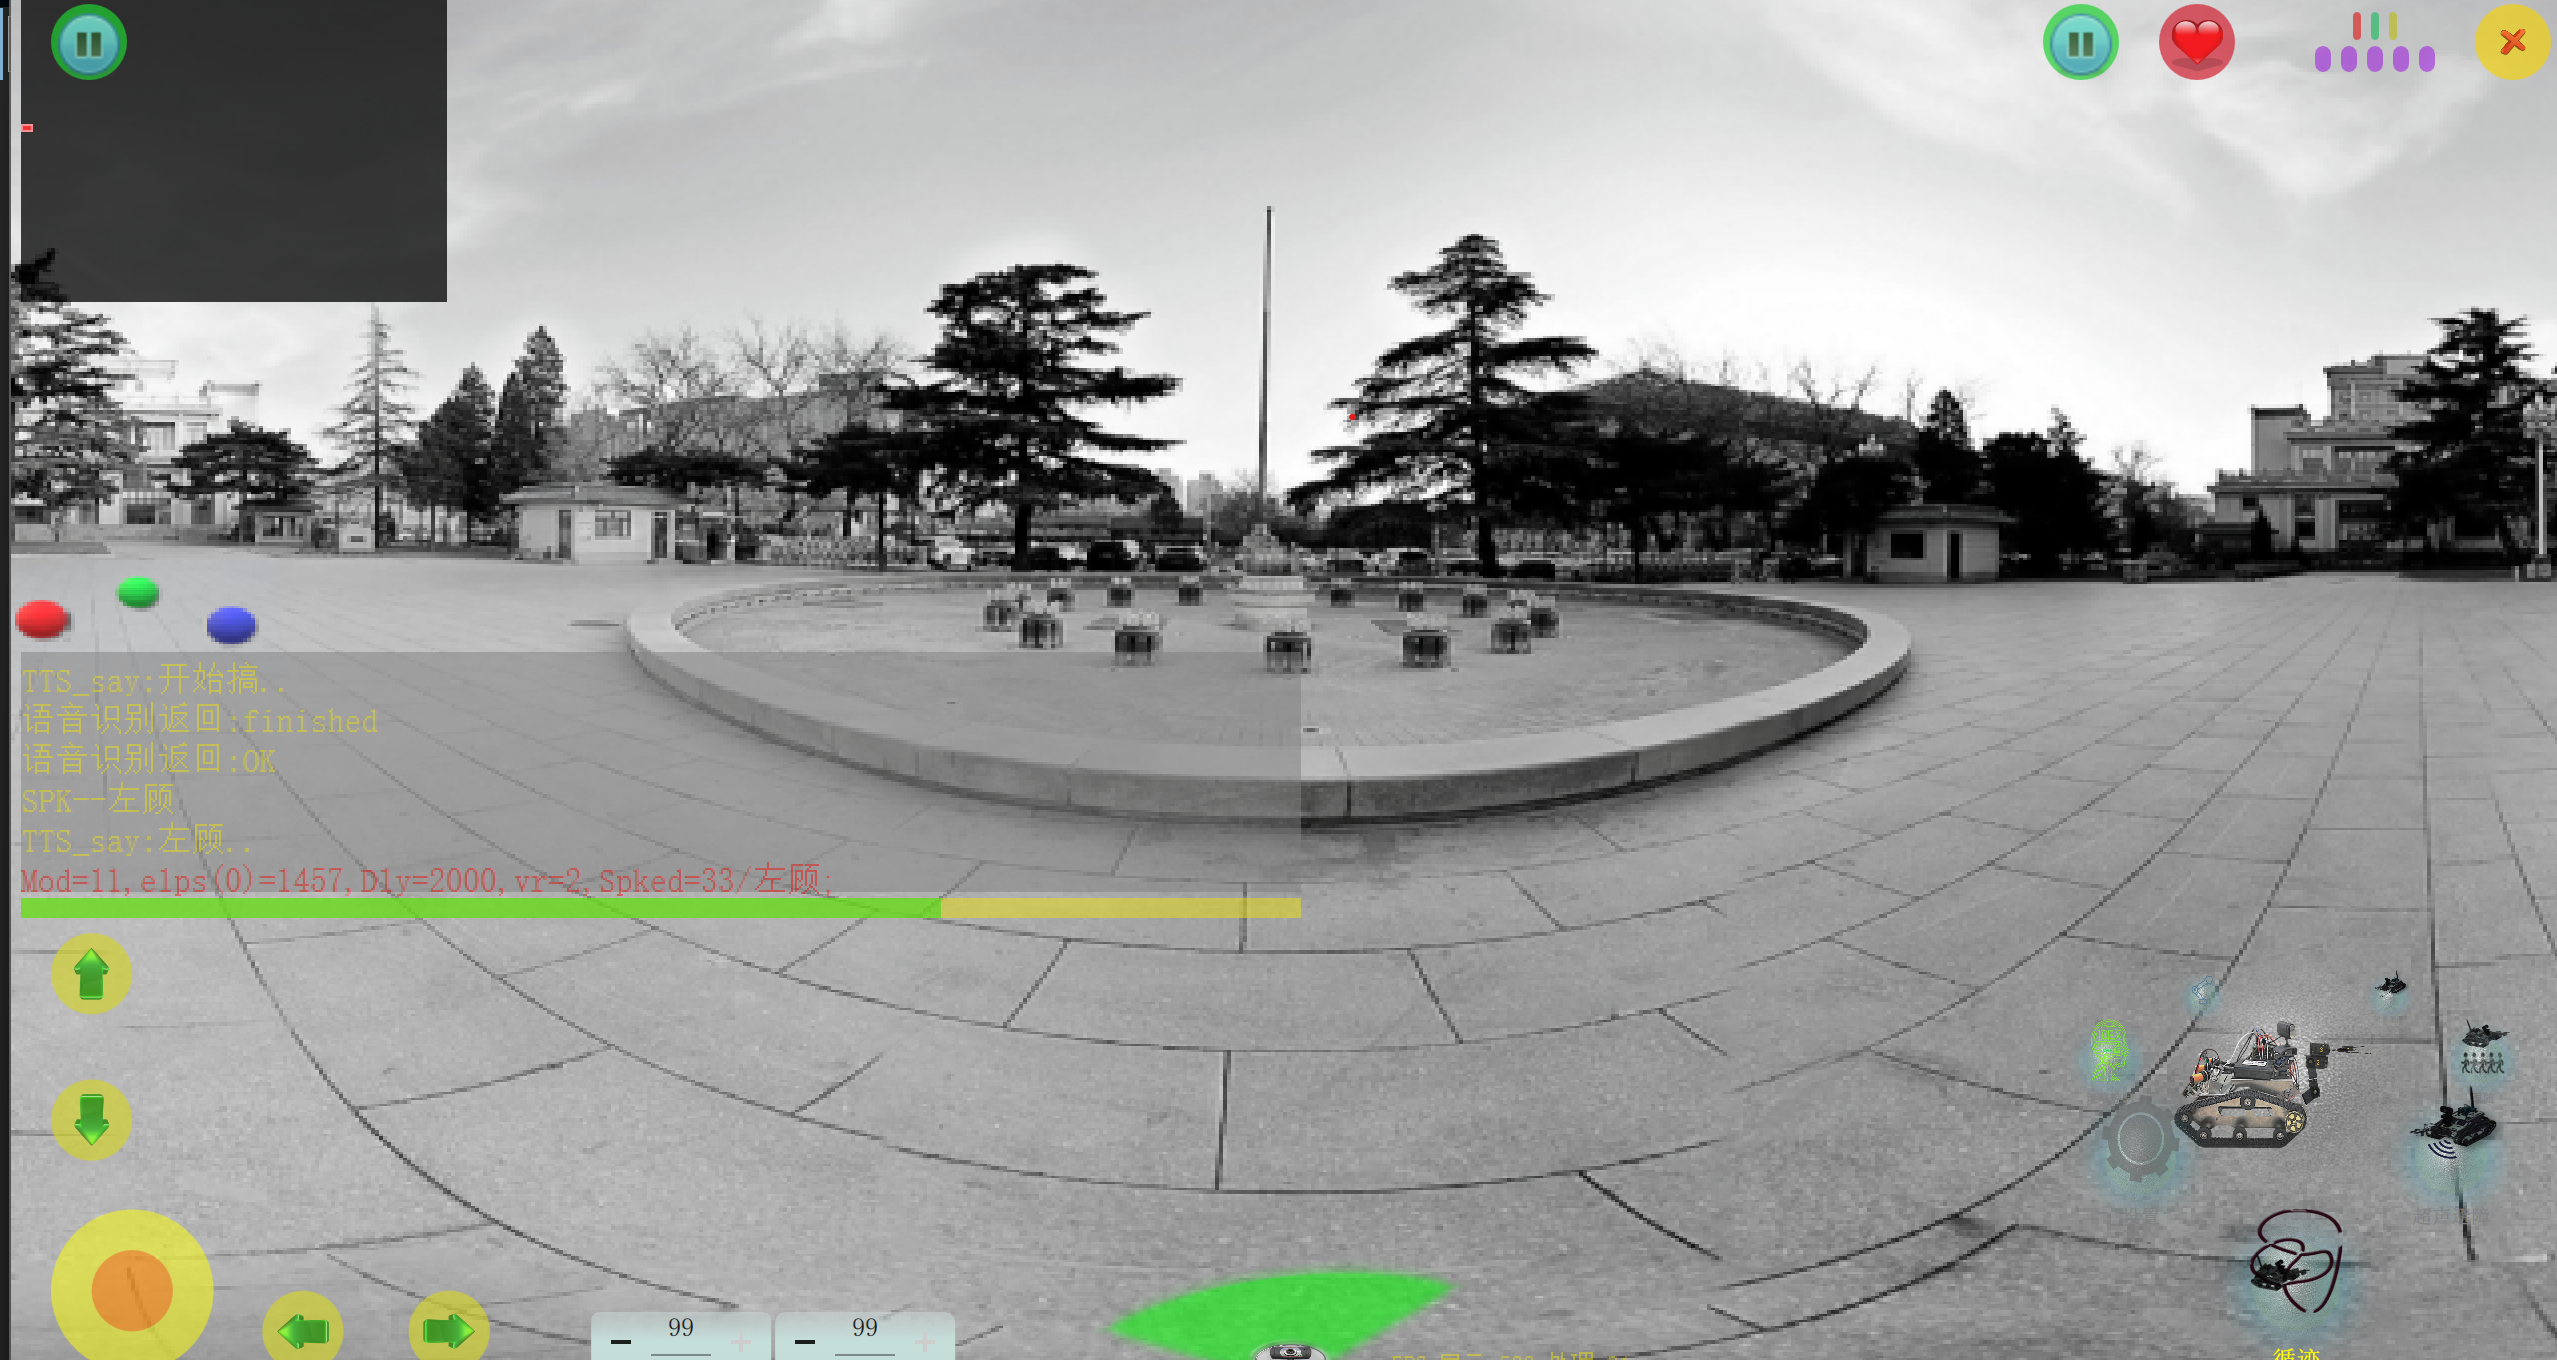
\includegraphics[width = .8\textwidth]{./figure/左顾右盼.png}
    \caption{左顾右盼}
\end{figure}
\begin{figure}[H]
    \centering
    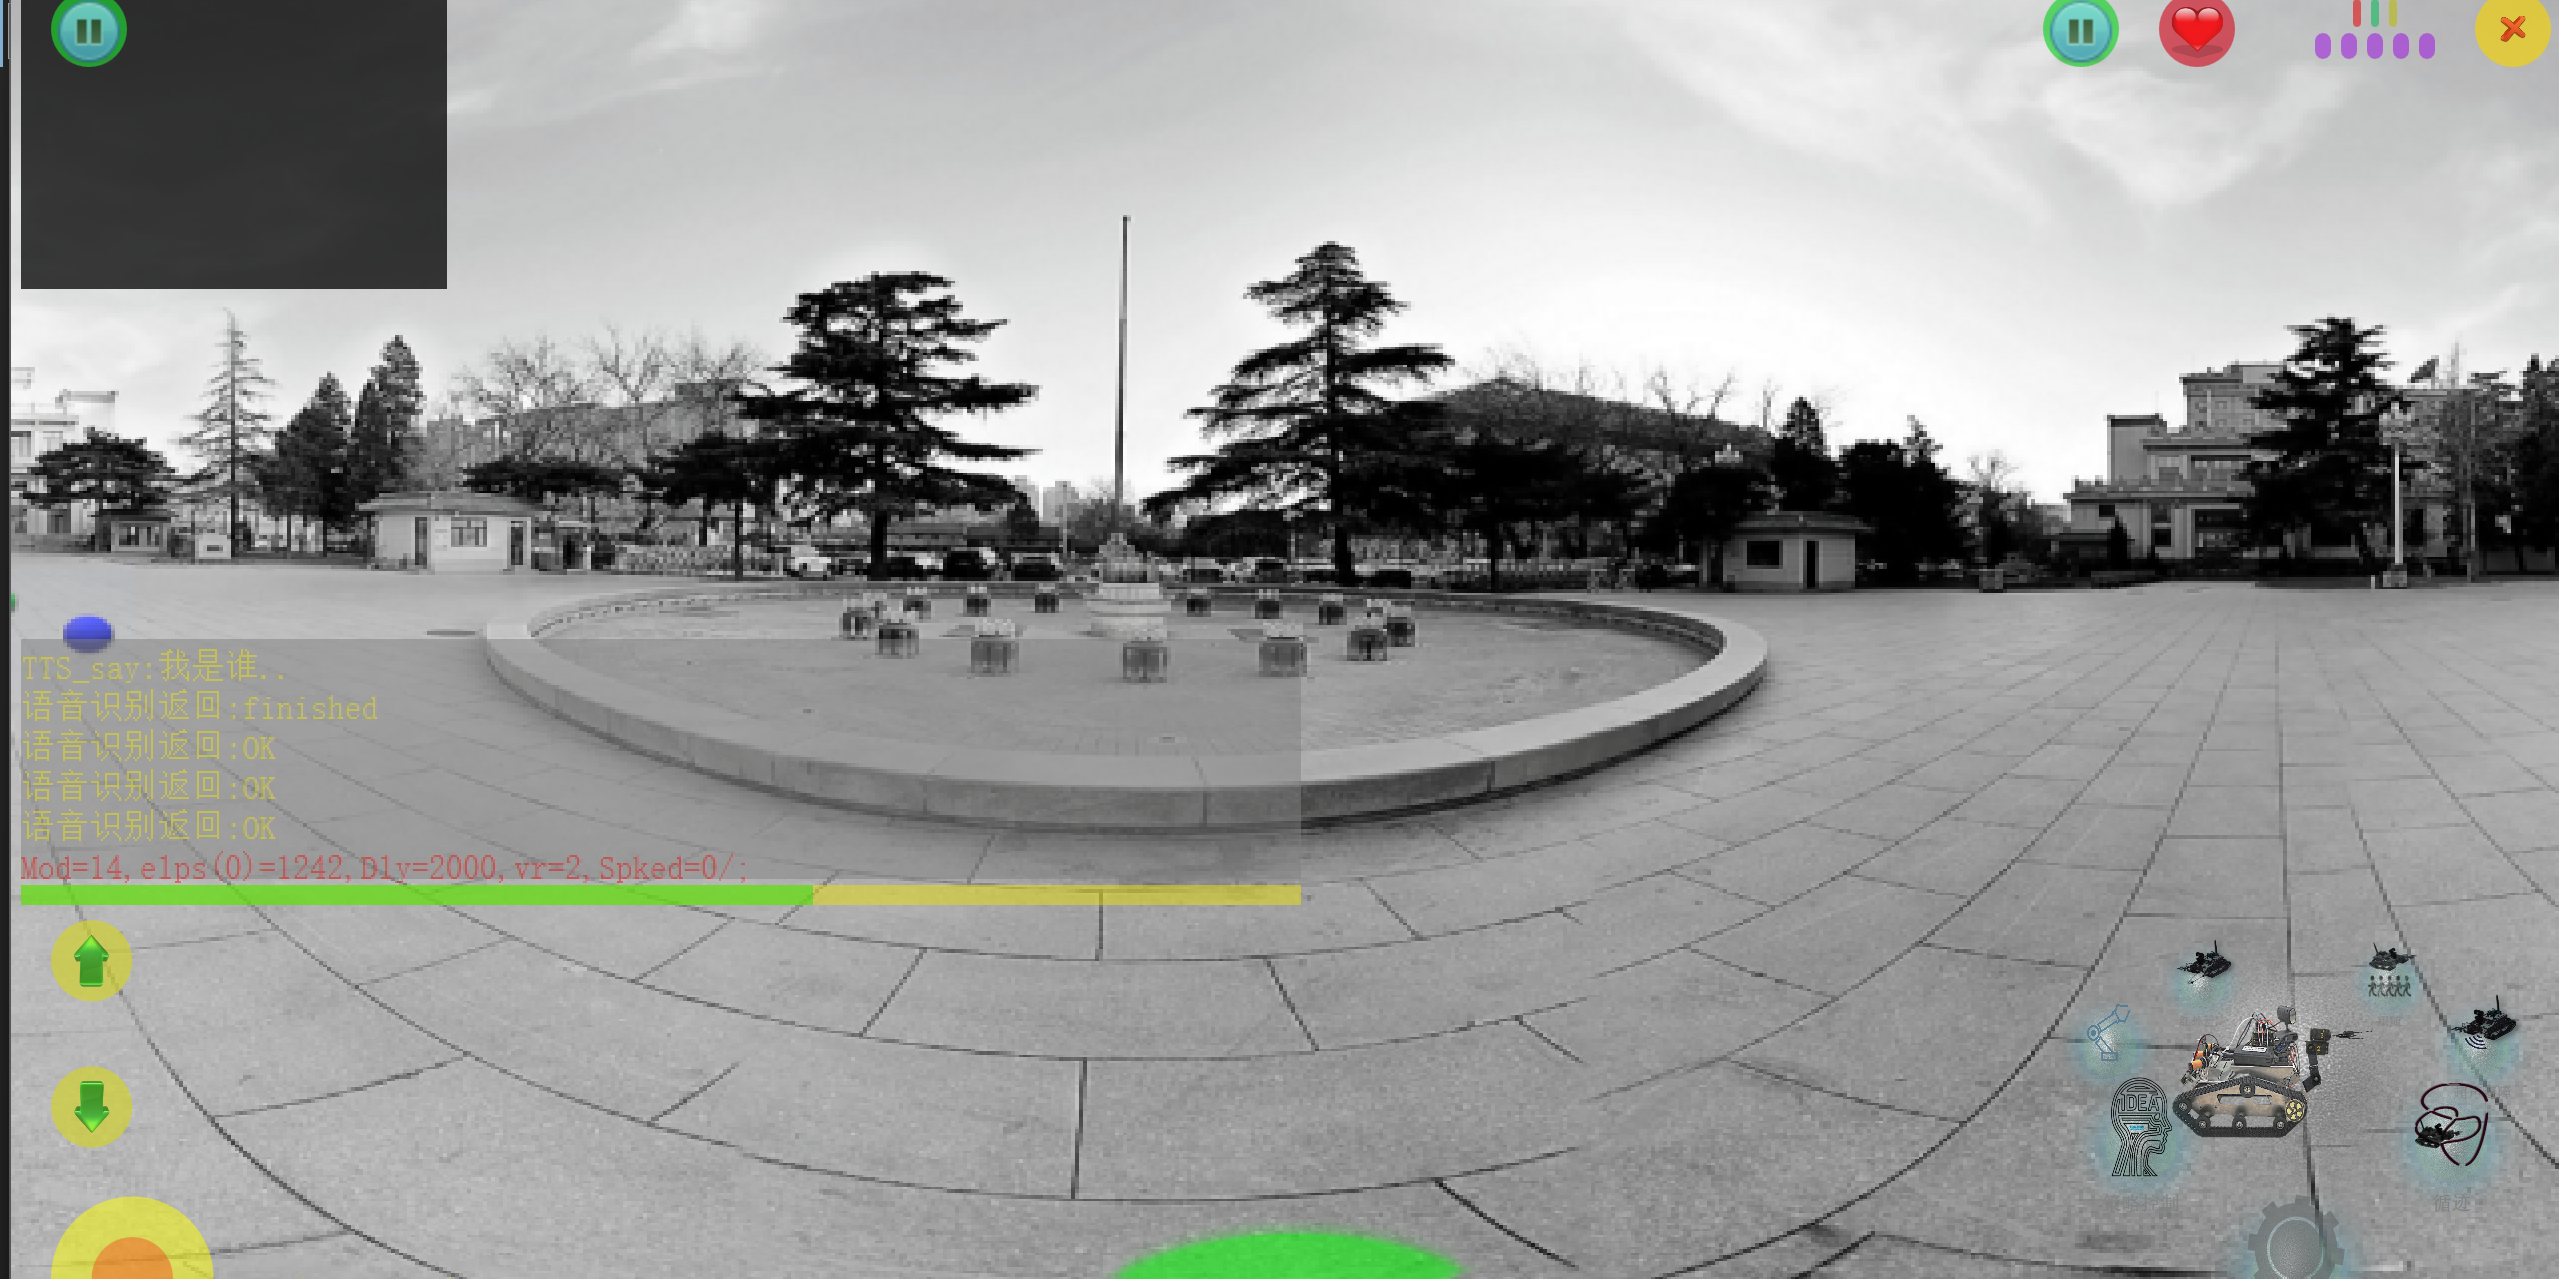
\includegraphics[width = .8\textwidth]{./figure/点头.png}
    \caption{点头}
\end{figure}
\begin{figure}[H]
    \centering
    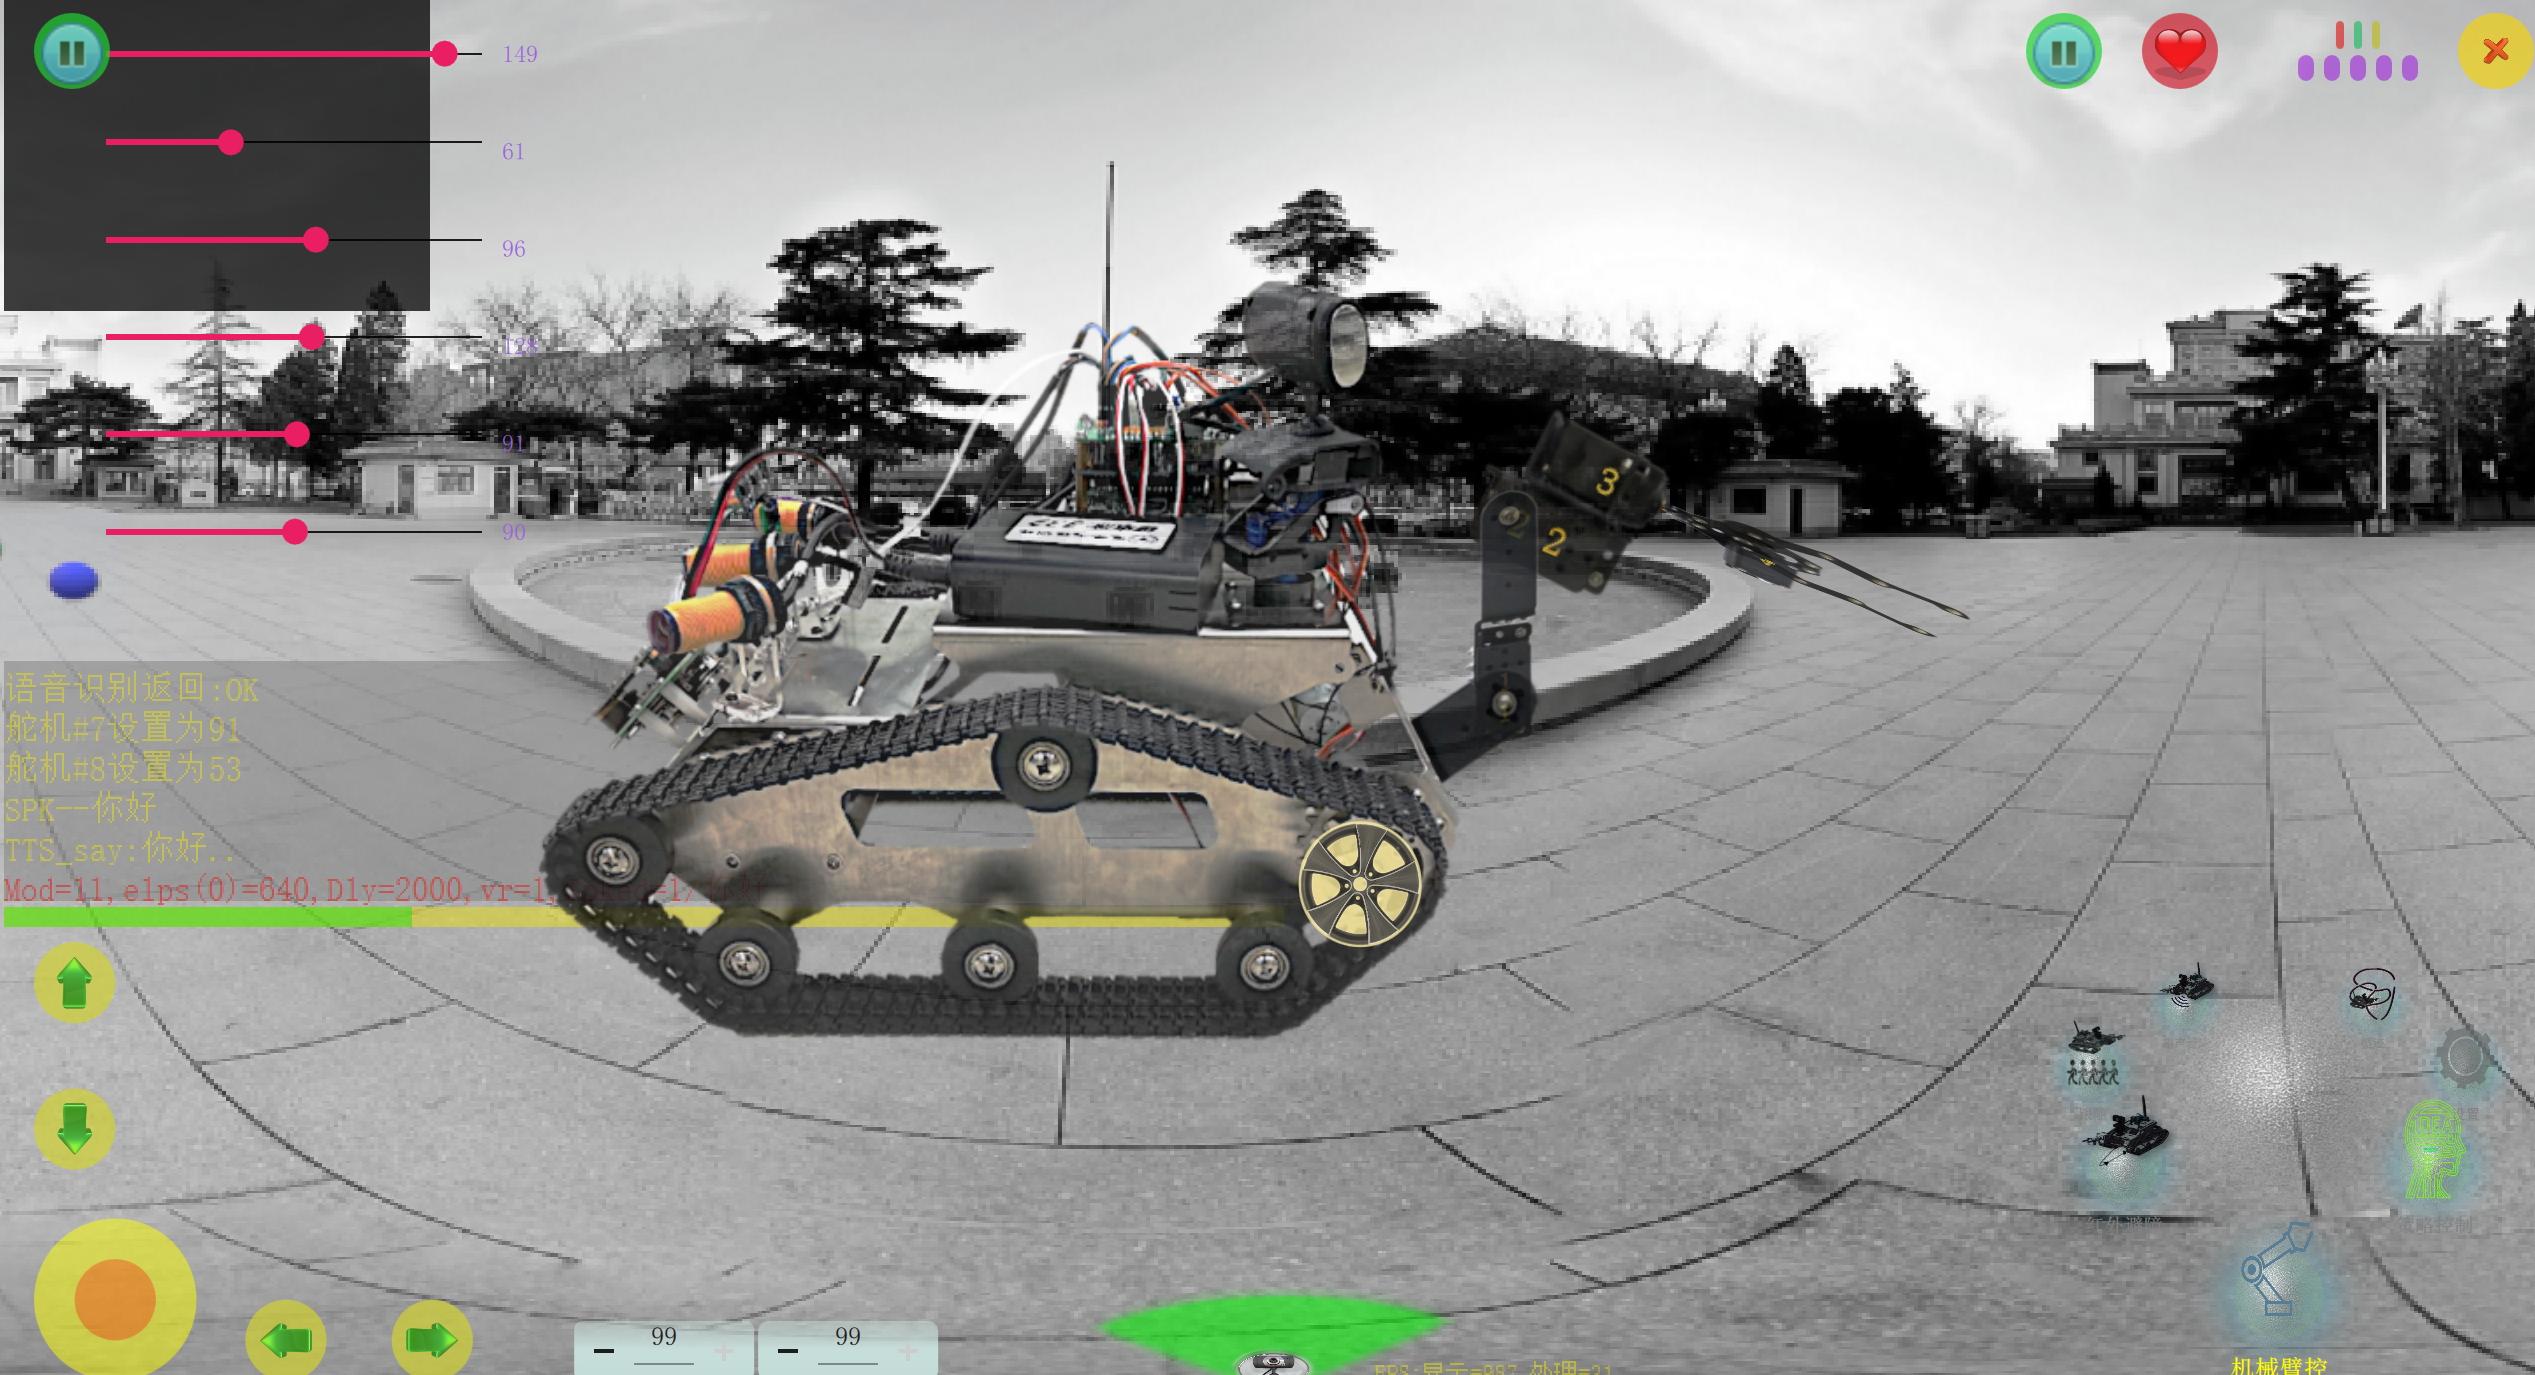
\includegraphics[width = .8\textwidth]{./figure/握手.png}
    \caption{握手}
\end{figure}
\begin{figure}[H]
    \centering
    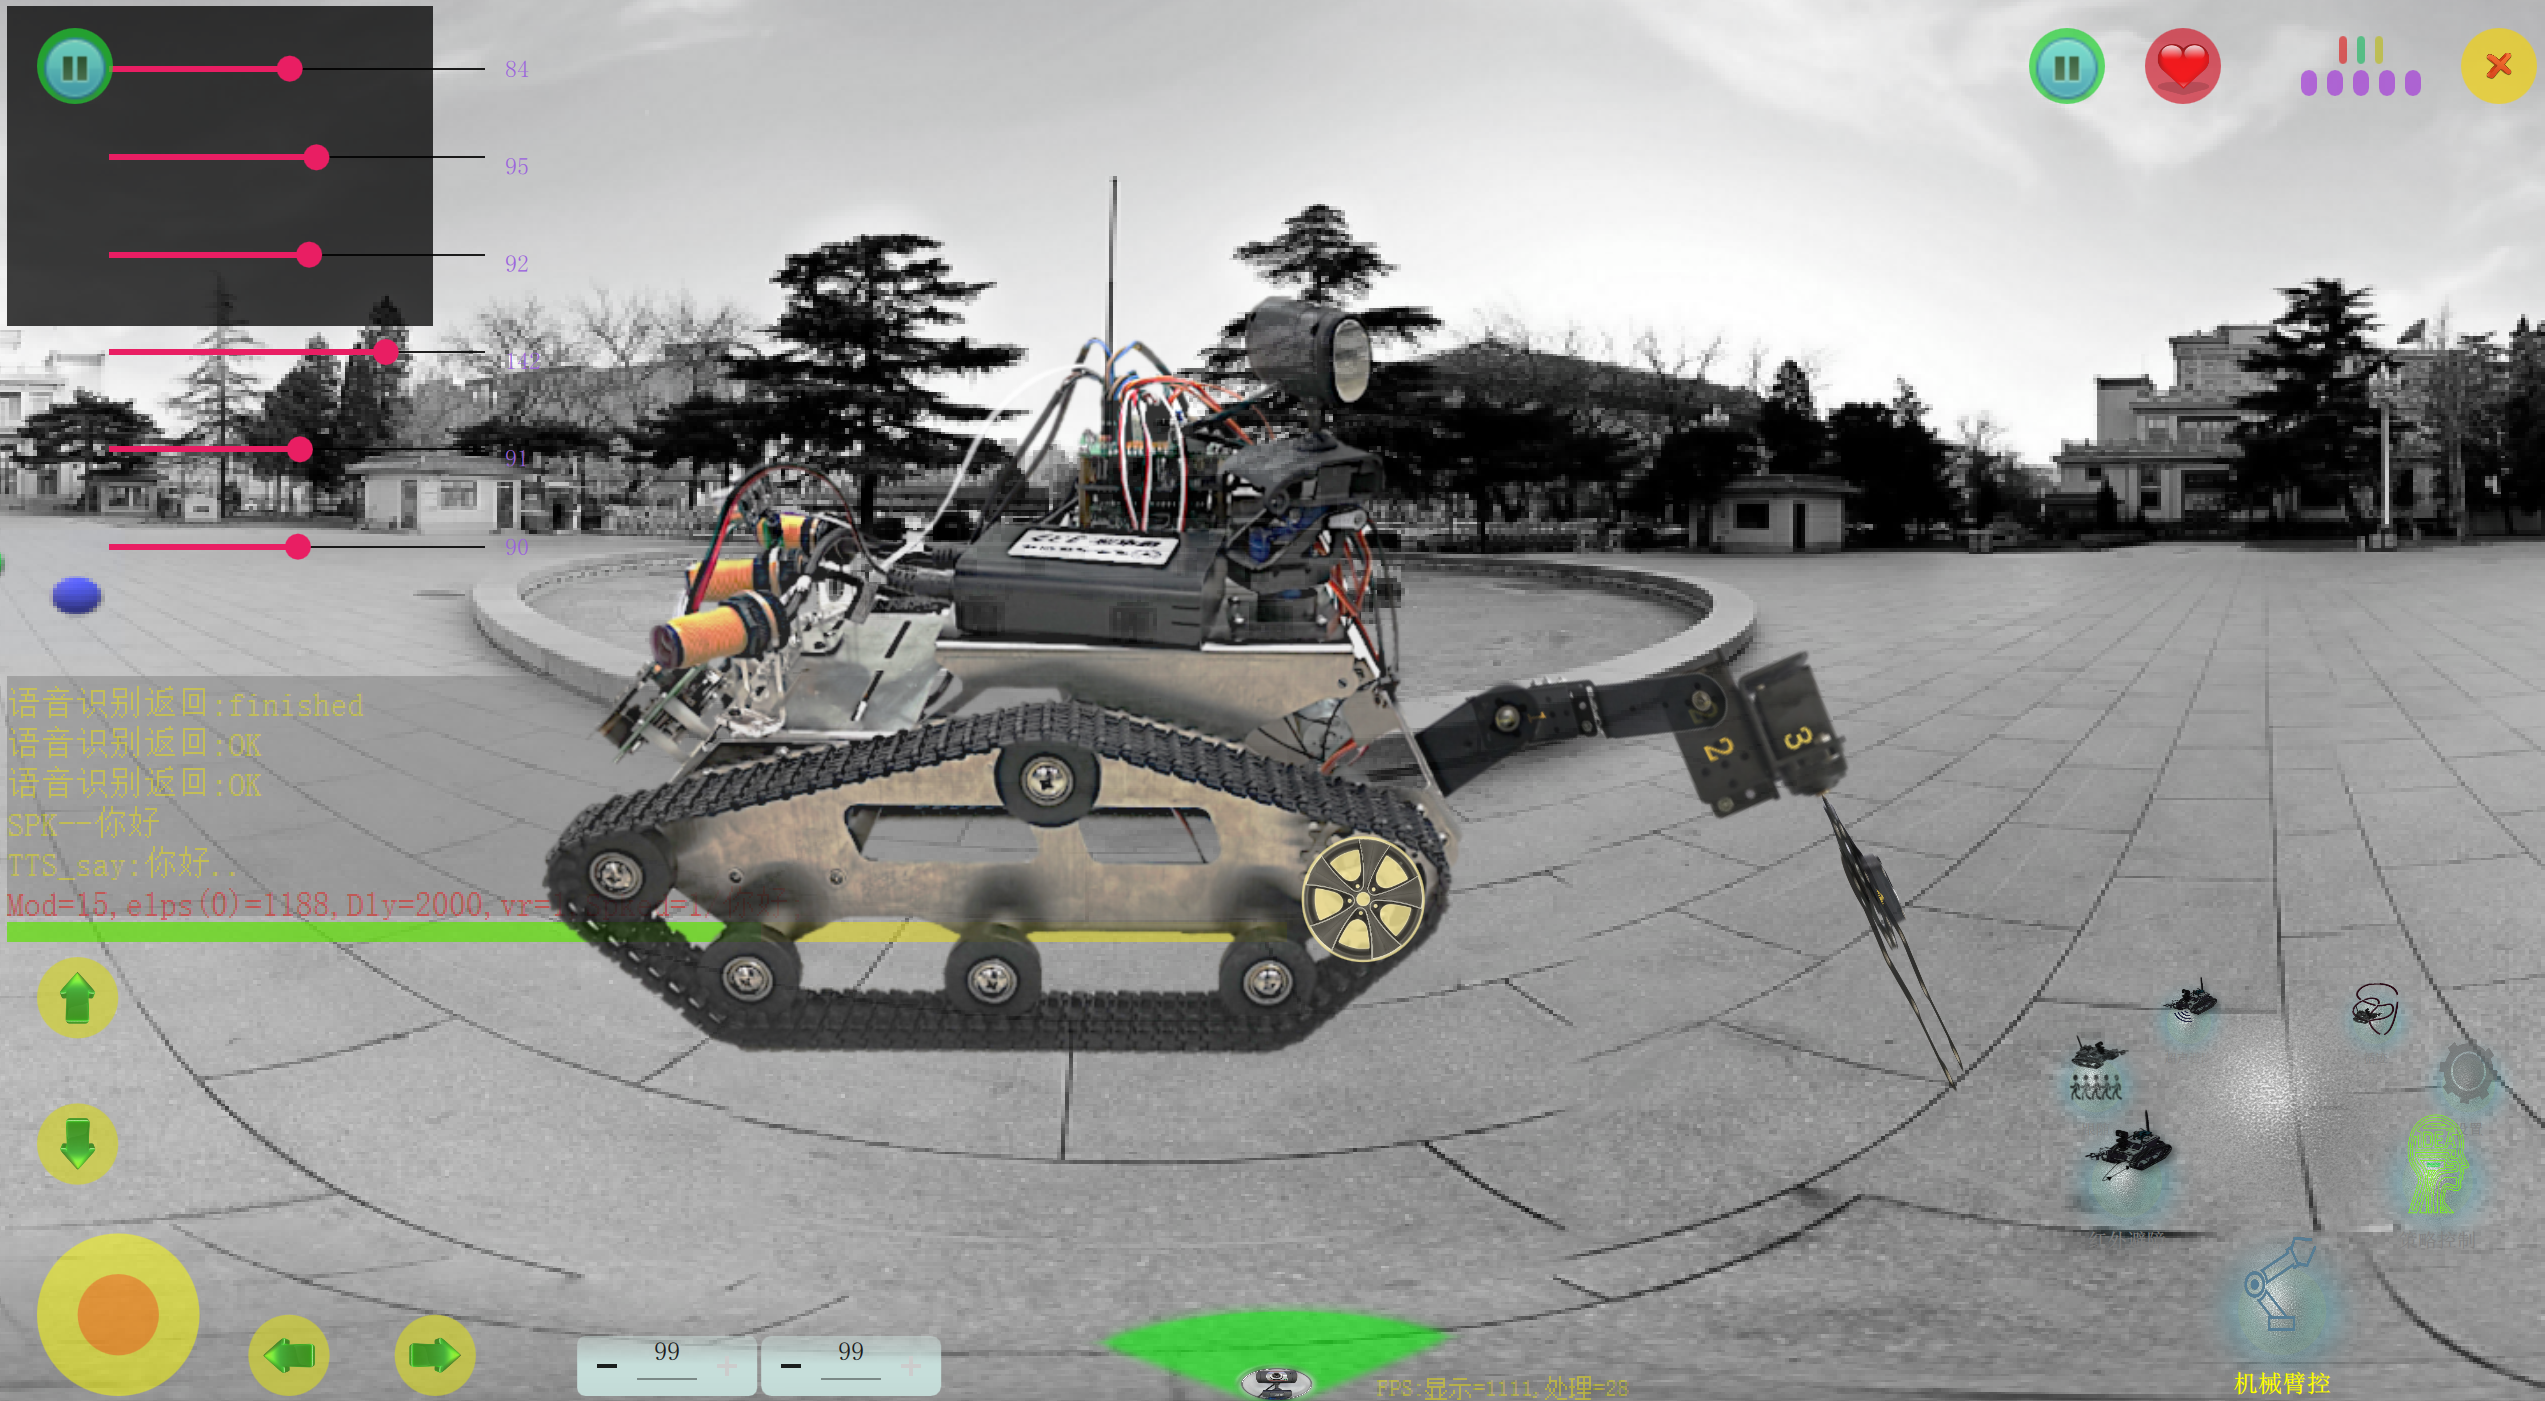
\includegraphics[width = .8\textwidth]{./figure/抓球.png}
    \caption{抓球}
\end{figure}
\end{document}